\documentclass{article}

\usepackage[T1]{fontenc}
\usepackage{microtype}
\usepackage{graphicx}
\usepackage{booktabs}
\usepackage{amsmath}
\usepackage{amssymb}
\usepackage{hyperref}
\setlength{\emergencystretch}{2em}

\newcommand{\theHalgorithm}{\arabic{algorithm}}

\usepackage[accepted]{mlsys2025}

\makeatletter
\renewcommand{\mlsys@appearing}{Copyright 2026 by the author.}
\renewcommand{\Notice@String}{\mlsys@appearing}
\makeatother

\hypersetup{
  pdftitle={What Training Data Should Lose: Local Extraction, Redaction, and Fail-Closed Gatekeeping},
  pdfauthor={Gege Ardiyansyah},
  pdfsubject={Systems for Machine Learning}
}

\mlsystitlerunning{What Training Data Should Lose: Local Extraction, Redaction, and Fail-Closed Gatekeeping}

\begin{document}

\twocolumn[
\mlsystitle{What Training Data Should Lose: Local Extraction, Redaction, and Fail-Closed Gatekeeping}

\begin{mlsysauthorlist}
\textbf{Gege Ardiyansyah}
\end{mlsysauthorlist}

\mlsystitlerunning{What Training Data Should Lose: Local Extraction, Redaction, and Fail-Closed Gatekeeping}
\mlsyskeywords{WebAssembly, conformal prediction, Learn-Then-Test, PII de-identification, document curation}

\vskip 0.3in

\begin{abstract}
Preparing institutional documents for AI retrieval or post-training requires stripping boilerplate, redacting sensitive fields, and filtering low-quality passages. In clinical, legal, and regulated settings, raw records cannot reach cloud preprocessing APIs, so the entire pipeline must run deterministically inside a local, auditable sandbox. We present \textbf{Versieve}, a document curation and conformal gatekeeping engine with no network egress by default. Its contribution is the release policy rather than the stack: a fail-closed three-way \texttt{KEEP}/\texttt{ABSTAIN}/\texttt{DROP} rule with a drop floor, operationalized on a zero-host-import WebAssembly kernel boundary and a $2{,}129$\,B single-header C99 core shared byte-identically across browser, Node.js, MCP, and C99 substrates. We evaluate Versieve across a $1{,}207$-document public benchmark suite (ICDAR-2019 FUNSD, PubMedQA, PubMed Central full-text PDFs, and \texttt{ai4privacy-200k}) and four runtime substrates on an 8\,GB RTX~4070 Laptop GPU. Deterministic ingestion extracts readable prose from all $8/8$ PMC PDFs ($8{,}134$ lines, $55{,}099$ words in $209.02$\,ms) without raster OCR and preserves $97.38\%$ of FUNSD word boxes under $512{\times}512$ overlapping tiles. Format-validated regular expressions recall $78.6\%$ ($110/140$) of contact, card, and IPv4 spans, $49.6\%$ ($118/238$) of bare person names, and $31.0\%$ ($180/580$) of the $26$ structured PII tags (out of the dataset's $56$ span categories), while a $334$-word exclusion lexicon reduces false-positive Title-Case hits on blind PubMedQA abstracts by $2.72\times$ ($5.46 \to 2.01$ per $1{,}000$ words). Above the regex layer, a 520-dimensional logistic gatekeeper calibrated via Learn-Then-Test (LTT) provides monotonic held-out risk control ($14.63\% \to 0.0\%$ conditional FPR) and fails closed cleanly at $\alpha=0.01$ when the unsafe calibration sample is below the theoretical floor ($n_{\text{cal,unsafe}}=206 < 299$, $\operatorname{BinomCDF}=0.1261 > 0.05$). Across runtime substrates, median process startup is $14.12$\,ms (C99) and $106.22$\,ms (Node+WASM) versus $12{,}917$\,ms for PyTorch+DuckDB. The gate's certificates are relative to the scanner-derived unsafe and safe labels, bounding what the redaction layer can catch rather than independent PII truth.
\end{abstract}
]

\section{Introduction}
\label{sec:intro}

Domain-specific retrieval and post-training pipelines ingest heterogeneous institutional documents, including scientific PDFs, Word reports, web pages, and scanned forms \citep{soldaini2024dolma,penedo2024fineweb}. Standard curation stacks often rely on hosted language models or cloud de-identification services \citep{ai4privacy2023,presidio2021}. For clinical, legal, and confidential enterprise corpora, however, transmitting raw source documents to external endpoints violates organizational or regulatory data-residency boundaries.

Running curation locally introduces a distinct systems challenge: the pipeline must start in milliseconds on standard laptops, replay and audit every redaction decision deterministically, and abstain rather than silently release sensitive records when a heuristic detector misses an unusual PII format.

We design and evaluate \textbf{Versieve}, a portable, zero-egress document preparation and retrieval stack organized across three explicit layers:
\begin{enumerate}
    \item \textbf{Interactive Web Workbench (RTIO):} A browser interface (\url{https://www.rtio.io/sandbox}) for inspecting documents, labeling customer-specific chunks, and launching local open-weight workflows without uploading files.
    \item \textbf{Portable Curation and Gatekeeping Engine (Versieve):} A shared deterministic core implementing PDF and \texttt{.docx} parsing, multi-stage deduplication, salted-pseudonym PII redaction, 520-dimensional feature extraction, and finite-sample Learn-Then-Test (LTT) conformal gatekeeping across the browser, Node.js CLI, Model Context Protocol (MCP) server, and a $2{,}129$\,B single-header C99 library (\texttt{include/versieve.h}).
    \item \textbf{Zero-Import WebAssembly Kernels:} Five standalone WASM binaries totaling $388{,}797$\,B, audited at load time to declare no host imports (a packaging and audit choice within the established WASM sandbox lineage, Section~\ref{sec:related}): \texttt{versieve\_clean.wasm} ($14{,}633$\,B) for text normalization, deduplication, and token-window chunking; \texttt{versieve\_graph.wasm} ($54{,}402$\,B) for Dual-CSR document knowledge graphs, personalized PageRank (PPR), GDPR Art.~17 blast-radius eviction, shortest paths, Tarjan SCC, and Louvain clustering; \texttt{versieve\_dl.wasm} ($60{,}096$\,B, $26$ \texttt{mle\_dl\_*} exports) for BitNet encoding, VeRA adapter training, and 64-dimensional needle retrieval \citep{wang2024bitnet,kopiczko2024vera,vaswani2017attention}; \texttt{versieve\_sql.wasm} ($55{,}635$\,B) for local SQL filtering and inner equi-joins; and \texttt{versieve\_media.wasm} ($204{,}031$\,B, $29$ exports) for archive, secret, audio, and visual sanitization evaluated in the companion multimodal study \citep{ardiyansyah2026multimodal}. Optical character recognition (OCR) is isolated in a separate \texttt{cactus.wasm} module ($1{,}240{,}671$\,B) that fails closed whenever local OCR weights are absent.
\end{enumerate}

\paragraph{Privacy boundaries.}
Privacy-leakage analyses establish that imperfect text scrubbing still permits memorization and inference of private attributes \citep{lukas2023pii,staab2024beyond}, which motivates calibrated attacker-based privacy auditing \citep{cpa2026auditing}. Consistent with those findings, the zero-egress claim covers user bytes (optional local model weights are fetched once, cached offline, and fail closed when absent), and the LTT certificates are scoped to detector-closed bounds, not adversarial privacy guarantees.

\paragraph{Scope of novelty.}
Individually, WebAssembly sandboxing \citep{haas2017wasm}, scholarly PDF glyph-map (CMap) parsing \citep{lo2020s2orc}, logistic regression, Learn-Then-Test \citep{angelopoulos2021ltt}, and regex-plus-lexicon redaction \citep{presidio2021} are established building blocks. Versieve contributes three things: (1)~a zero-host-import WASM kernel boundary whose declared import surface is verified empty at load time and shared byte-identically across the C99, Node.js, and browser substrates; (2)~a $2{,}129$\,B single-header C99 core executing the JavaScript engine's ingestion, redaction, and 520-dimensional logistic scoring identically in float32 C99 (Section~\ref{sec:substrates}); and (3)~the fail-closed three-way release policy (Sections~\ref{sec:ltt} and~\ref{sec:ltt-multi}): a KEEP/ABSTAIN/DROP decision rule with a drop floor and a multi-axis conjunction that refuses to certify any threshold the calibration sample cannot support. The contribution is the release policy and its operationalization, not the LTT statistic or the sandbox itself.

\begin{table}[t]
\caption{Summary of Versieve capabilities, verified measurements, and explicit operating boundaries.}
\label{tab:scope}
\vskip 0.08in
\begin{center}
\resizebox{\columnwidth}{!}{%
\begin{tabular}{lp{1.55in}p{1.35in}}
\toprule
\textbf{Subsystem} & \textbf{Verified Behavior} & \textbf{Operating Boundary} \\
\midrule
Web/Link Capture & Strips $53.7\%$ HTML boilerplate in $1.345$\,ms; blocks private IPs & Live remote fetch requires outbound network \\
PDF \& Word Files & Extracts \texttt{.docx} in $2.477$\,ms; $8/8$ PMC PDFs in $209.02$\,ms & Image-only PDFs require local OCR weights \\
Dedupe \& Manifest & SHA-256 + 3-gram Jaccard ($\ge 0.85$); signed provenance hash & Per-shard in-memory ring, not TB streaming \\
Conformal Gate & \texttt{safe} certifies at $\tau=0.55$; fails closed when $n_{\text{cal}}$ is too small & Small calibration sets yield conservative abstention \\
Local Substrates & C99 spawn $14.12$\,ms; NumPy wins shared logistic ($0.207$\,ms) & Warm compute varies by kernel architecture \\
\bottomrule
\end{tabular}%
}
\end{center}
\vskip -0.14in
\end{table}

Table~\ref{tab:scope} summarizes each subsystem alongside its explicit operating boundary, Figure~\ref{fig:redaction-arch} traces the end-to-end flow, and Section~\ref{sec:related} positions the system against related work.

\begin{figure*}[t]
\centering
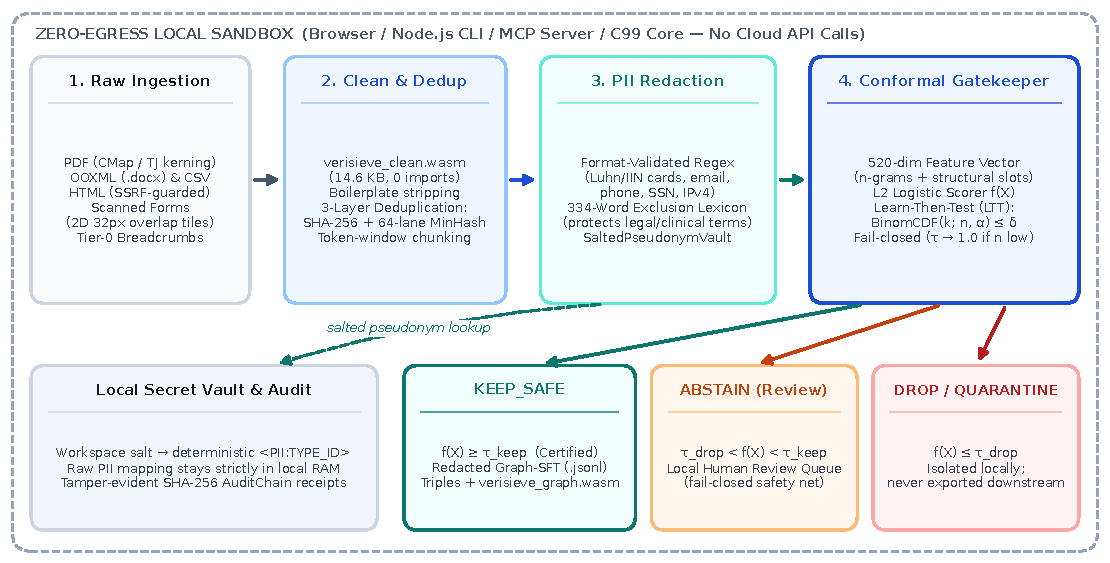
\includegraphics[width=0.98\textwidth]{figs/fig0-redaction-architecture.pdf}
\caption{End-to-end zero-egress Versieve architecture: deterministic parsing, zero-import WASM deduplication (\texttt{versieve\_clean.wasm}), format-validated PII redaction backed by a local-only \texttt{SaltedPseudonymVault} and a $334$-word exclusion lexicon, and fail-closed LTT routing to \texttt{KEEP\_SAFE} exports, \texttt{ABSTAIN} review, or \texttt{DROP} quarantine.}
\label{fig:redaction-arch}
\end{figure*}

\section{Deterministic Document Ingestion and Layout Preservation}
\label{sec:ingestion}

Reliable downstream filtering and retrieval depend on converting raw binary and markup formats into clean, provenance-tracked text blocks without silently dropping content.

\subsection{HTML Stripping, OOXML Parsing, and Deduplication}
On the portable ingestion micro-benchmark, Versieve strips raw HTML boilerplate by $53.7\%$ ($503$\,B raw HTML to $233$\,B clean prose) in $1.345$\,ms, extracts $150$ characters from a $295$\,B native \texttt{.docx} OOXML container (including bit-3 ZIP data-descriptor archives) in $2.477$\,ms, and executes two-stage deduplication (exact SHA-256 plus 3-gram Jaccard similarity at $\ge 0.85$) across $5$ inputs into $4$ unique chunks in $0.554$\,ms. Emitting a signed manifest over $2$ sources and $50$ tokens (SHA-256 prefix \texttt{2de7618c79d41782}) completes the combined four-stage micro-benchmark in $5.393$\,ms.

\subsection{Native PDF CMap and Kerning Reconstruction}
Many scientific and regulatory PDFs embed custom glyph encodings rather than plain ASCII strings. Versieve's native parser (\texttt{extractPdfDiagnostics}) scans each PDF content stream in a single pass, resolves scoped 1-byte and 2-byte \texttt{/ToUnicode} CMap tables (\texttt{beginbfchar} and \texttt{beginbfrange}), and inserts word spaces whenever a PDF \texttt{TJ} operator specifies a negative kerning displacement of $\le -110$ glyph units.

Across all $8$ open-access PubMed Central (PMC) clinical PDFs in our evaluation suite, $7$ contain embedded \texttt{/ToUnicode} CMap streams and $2$ contain hex-encoded strings ($1$ and $57$ hex-decoded lines). Versieve recovers readable prose from all $8/8$ documents ($8{,}134$ lines and $55{,}099$ words) in $209.02$\,ms total ($26.13$\,ms per paper; range $8.42$\,ms to $64.54$\,ms) without invoking raster OCR.

\subsection{2D Overlapping Tiling for Scanned Forms}
When documents exist only as page images, naive downscaling destroys small form fields before an OCR model can read them. On all $199$ scanned forms in the ICDAR-2019 FUNSD dataset \citep{jaume2019funsd} ($30{,}595$ annotated word boxes), we evaluate how many word boxes remain geometrically legible ($\ge 8$\,px height and $\ge 4$\,px width after scaling) under five rasterization strategies (Table~\ref{tab:funsd}).

\begin{table}[t]
\caption{Geometric word-box survival on $199$ ICDAR-2019 FUNSD forms ($30{,}595$ boxes; legibility threshold $\ge 8{\times}4$\,px).}
\label{tab:funsd}
\vskip 0.08in
\begin{center}
\resizebox{\columnwidth}{!}{%
\begin{tabular}{lrrl}
\toprule
\textbf{Rasterization Strategy} & \textbf{Survived} & \textbf{Rate} & \textbf{Primary Failure Mode} \\
\midrule
Capped at 8 Reads & $1{,}592$ & $5.20\%$ & Read budget drops dense fields \\
Untiled $512{\times}512$ Scale & $6{,}281$ & $20.53\%$ & Small labels shrink below $8{\times}4$\,px \\
Horizontal 1D Bands ($512$\,px) & $21{,}811$ & $71.29\%$ & Aspect compression and seam cuts \\
2D Grid (Zero Overlap) & $28{,}283$ & $92.44\%$ & $4.94\%$ lost on tile boundaries \\
\textbf{2D Grid ($32$\,px Overlap)} & $\mathbf{29{,}793}$ & $\mathbf{97.38\%}$ & Avg.\ $6$ tiles/form ($6.29$\,ms scan) \\
\bottomrule
\end{tabular}%
}
\end{center}
\vskip -0.14in
\end{table}

Untiled $512{\times}512$ downscaling preserves only $20.53\%$ of word boxes, and a non-overlapping 2D grid still severs $4.94\%$ along tile seams; adding a $32$\,px overlap raises geometric survival to $97.38\%$ ($29{,}793 / 30{,}595$ boxes; Table~\ref{tab:funsd}).

\section{Related Work}
\label{sec:related}

\paragraph{WebAssembly and edge-data isolation.}
WebAssembly is an established sandboxing substrate \citep{haas2017wasm} whose performance and isolation trade-offs against native code are well characterized \citep{jangda2019notsofast}. Versieve treats WASM sandboxing as inherited: its zero-host-import kernels are a packaging and audit choice within that lineage. The audit boundary buys a load-time check that a kernel's declared import surface is empty, byte-identically across C99, Node.js, and browser substrates, as the implementation vehicle for the fail-closed release policy; no audited prior art establishes zero host imports as either novel or routine, so we claim auditability, not priority.

\paragraph{Local de-identification and curation.}
Microsoft Presidio \citep{presidio2021} is the standard pluggable de-identification layer, and local-first curation and redaction pipelines with provenance tracking \citep{bhattacharjee2026curatorkit,redakto2026incognito} target the same no-egress constraint. The neural tagger Versieve benchmarks as an alternative first pass, GLiNER-Edge, descends from GLiNER \citep{zaratiana2024gliner}. Versieve contributes the statistically certified release policy above whichever detector is plugged in, not a new detector.

\paragraph{Conformal selective prediction and LTT.}
Learn-Then-Test \citep{angelopoulos2021ltt} and conformal risk control \citep{angelopoulos2022crc} supply the finite-sample risk-control machinery, alongside risk-controlling prediction sets \citep{bates2021distributionfree} and conformal abstention \citep{abbasiyadkori2024abstention}. LTT is inherited wholesale; the gate in this paper adds only the three-way decision rule, the drop floor, and fail-closed certificate behavior around it.

\paragraph{PDF and layout extraction.}
Scholarly-PDF text recovery via glyph-map (CMap) parsing and layout analysis is established practice: machine-learned PDF parsers underpin curation corpora such as S2ORC \citep{lo2020s2orc}, and overlapped image tiling is a standard OCR preprocessing technique. Versieve's CMap and kerning parser is a dependency-free implementation of these techniques, and the 2D-tiled results of Section~\ref{sec:ingestion} measure that implementation, not a new extraction method.

\section{Evaluation Corpus and Hardware Testbed}
\label{sec:datasets}

Core curation, PII disambiguation, conformal calibration, and substrate benchmarks run over a unified $1{,}207$-document public corpus combining real archival and biomedical documents with span-annotated synthetic PII records (Table~\ref{tab:datasets}). Under the format-validated scanner, $826$ documents are labeled unsafe and $381$ safe ($68.43\%$ unsafe prevalence). These labels are scanner-derived: they are independent of scanner judgment only where a dataset supplies ground-truth PII spans (\texttt{ai4privacy-200k}). A conformal certificate therefore means agreement with the format-validated labeling rule, not independent PII truth; the $31.0\%$ ($180/580$) all-tag recall of Section~\ref{sec:pii} measures the scanner against \texttt{ai4privacy}'s human labels and bounds what the gate can catch, and the dataset's remaining free-form span categories are not counted toward the recall denominator.

\begin{table}[t]
\caption{Public benchmark corpus ($1{,}207$ documents; $826$ unsafe, $381$ safe under format-validated labeling).}
\label{tab:datasets}
\vskip 0.08in
\begin{center}
\resizebox{\columnwidth}{!}{%
\begin{tabular}{llll}
\toprule
\textbf{Dataset} & \textbf{Provenance} & \textbf{Docs} & \textbf{Evaluation Role} \\
\midrule
ICDAR FUNSD \citep{jaume2019funsd} & Real scanned forms & $199$ & $30{,}595$ word boxes; tiling geometry \\
\texttt{ai4privacy-200k} \citep{ai4privacy2023} & Synthetic English & $500$ & $56$-tag dataset; $26$ structured tags evaluated \\
PubMedQA \citep{jin2019pubmedqa} & Real clinical abstracts & $500$ & $250/250$ lexicon split; Needle QA \\
PMC full text \citep{miu_2017_pmc5773420} & Real clinical PDFs & $8$ & $8{,}134$ lines / $55{,}099$ words \\
\midrule
\textbf{Combined Suite} & \textbf{Real + Synthetic} & $\mathbf{1{,}207}$ & \textbf{$826$ unsafe / $381$ safe ($68.43\%$)} \\
\bottomrule
\end{tabular}%
}
\end{center}
\vskip -0.14in
\end{table}

\paragraph{Hardware and Software Environment.}
All benchmarks and GPU ablations ran locally on a single laptop: AMD Ryzen~7 7840HS ($8$ cores / $16$ threads), $31.3$\,GB RAM, NVIDIA GeForce RTX~4070 Laptop GPU ($8$\,GB VRAM), Windows~11 Home, Node.js v24.13.1, GCC~14.2.0 (MSYS2, C99 \texttt{-O3} binary $135{,}025$\,B), Python~3.12.4, NumPy~2.4.3, DuckDB~1.5.5, PyTorch~2.10.0+cpu (CPU substrate trials), and PyTorch~2.10.0+cu128 (local GPU LoRA training and inference).

\paragraph{Artifact availability.}
Every table in this paper is emitted by a checked-in runner in the project repository (\url{https://github.com/gegearsyah/versieve}) at commit \texttt{1e35603}; the benchmark manifests, prompts, and result JSON files are included with the submission, and the manifest lists each of the eight PMC identifiers (the Table~\ref{tab:datasets} citation is representative).

\section{PII Disambiguation and the Deterministic Regex Ceiling}
\label{sec:pii}

\begin{figure*}[t]
\centering
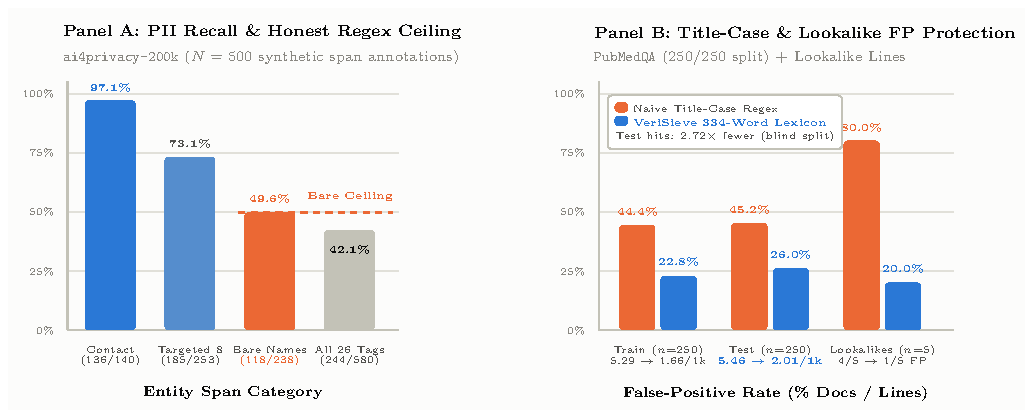
\includegraphics[width=0.96\textwidth]{figs/fig2-pii-disambiguation.pdf}
\caption{Format-validated PII scanning recall and false-positive reduction. \textbf{Panel A:} Recall by pattern class on $500$ \texttt{ai4privacy-200k} records. \textbf{Panel B:} Exclusion-lexicon reduction of false-positive Title-Case matches on the blind PubMedQA split (values in Section~\ref{sec:pii}).}
\label{fig:pii}
\end{figure*}

Regular-expression PII scrubbers face a sharp precision--recall trade-off on scientific and legal documents: aggressive Title-Case rules corrupt domain terminology (such as anatomical names, statistical methods, or statutory headings), while overly narrow patterns miss unprefixed human names and loosely formatted identifiers.

Versieve addresses precision in two ways: credit-card and financial identifier rules enforce Luhn checksum and Issuer Identification Number (IIN) validation so that arbitrary 16-digit scientific constants or grant IDs are not masked, and a pre-committed $334$-word exclusion lexicon (\texttt{EXCLUDED\_NAME\_WORDS}) suppresses common capitalized non-person phrases. On the held-out blind half of PubMedQA ($250$ clinical abstracts, $63{,}739$ words), the exclusion lexicon cuts false-positive Title-Case matches from $348$ ($5.46$ per $1{,}000$ words; $45.2\%$ of documents) down to $128$ ($2.01$ per $1{,}000$ words; $26.0\%$ of documents), a $2.72\times$ reduction (Figure~\ref{fig:pii}, Panel~B). On the development half ($62{,}620$ words), hits similarly decline from $5.29$ to $1.66$ per $1{,}000$ words ($44.4\% \to 22.8\%$ of documents), and false alarms on a five-item technical lookalike suite drop from $4/5$ to $1/5$.

At the same time, evaluating the validated scanner against ground-truth spans on $500$ \texttt{ai4privacy-200k} records exposes a clear recall ceiling (Figure~\ref{fig:pii}, Panel~A): recall is $78.6\%$ ($110/140$) on contact, card, and IPv4 spans, $62.8\%$ ($159/253$) across the eight targeted identifier patterns, $49.6\%$ ($118/238$) on bare unprefixed person names, and $31.0\%$ ($180/580$) across all $26$ structured privacy tags (which include free-form addresses, employers, and usernames).

\begin{table}[t]
\caption{External NER baselines on the identical $500$ \texttt{ai4privacy-200k} records ($580$ structured $26$-tag spans; $238$ bare-name spans; character-offset overlap with Wilson $95\%$ intervals; seed-$42$, $1{,}000$-resample bootstrap F1). Under the exact value-substring rule of Figure~\ref{fig:pii}, Versieve regex recalls $31.0\%$ ($180/580$).}
\label{tab:external-ner}
\vskip 0.08in
\begin{center}
\resizebox{\columnwidth}{!}{%
\begin{tabular}{lrrrrr}
\toprule
\textbf{Detector} & \textbf{26-Tag Rec.\ [95\% CI]} & \textbf{PII Prec.\ [95\% CI]} & \textbf{26-Tag F1} & \textbf{Bare Name} & \textbf{Med.\ ms} \\
\midrule
Versieve Regex & $35.17\%$ [$31.40, 39.14$] & $93.10\%$ [$90.55, 94.99$] & $51.06\%$ & $49.58\%$ ($118/238$) & -- \\
Presidio (\texttt{en\_core\_web\_lg}) & $\mathbf{64.48\%}$ [$60.50, 68.27$] & $\mathbf{93.95\%}$ [$92.08, 95.41$] & $\mathbf{76.48\%}$ & $\mathbf{87.39\%}$ ($208/238$) & $11.82$ \\
GLiNER-Edge v1.0 (INT8) & $62.41\%$ [$58.40, 66.26$] & $89.66\%$ [$87.61, 91.40$] & $73.60\%$ & $86.13\%$ ($205/238$) & $25.18$ \\
\bottomrule
\end{tabular}%
}
\end{center}
\vskip -0.14in
\end{table}

To separate the regex limit from task difficulty, Table~\ref{tab:external-ner} benchmarks Microsoft Presidio (\texttt{presidio-analyzer}~2.2.366, \texttt{spacy}~3.8.18, \texttt{en\_core\_web\_lg}~3.8.0 at threshold $0.50$) and Apache-2.0 \texttt{gliner-pii-edge-v1.0} ($45.8$\,MB INT8 ONNX, \texttt{onnxruntime}~1.26.0, threshold $0.40$) on the identical $500$ records and $580$ structured spans. Under uniform character-offset overlap, 26-tag recall rises from $35.17\%$ ($204/580$) for regex to $64.48\%$ ($374/580$; bootstrap F1 $76.48\%$ [$73.49\%, 79.44\%$]) for Presidio and $62.41\%$ ($362/580$; F1 $73.60\%$ [$70.83\%, 76.45\%$]) for GLiNER-Edge, bare-name recall to $87.39\%$ and $86.13\%$, and full 56-tag recall over $1{,}556$ spans to $50.00\%$, $64.33\%$, and $33.55\%$ respectively. Because neither deterministic regex nor neural span taggers achieve zero residual misses on unstructured prose, Versieve treats span detection as a pluggable first-pass redactor and places a statistically calibrated gatekeeper above it.

\section{Fail-Closed Conformal Gatekeeping}
\label{sec:ltt}

\begin{figure*}[t]
\centering
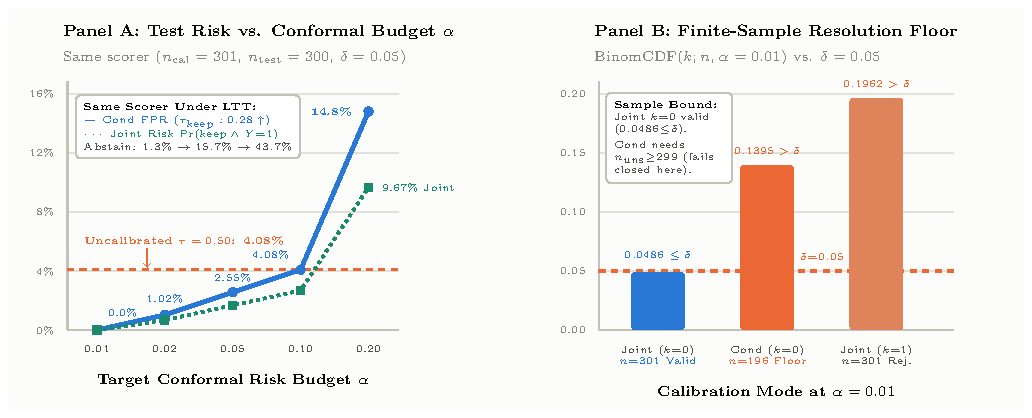
\includegraphics[width=0.96\textwidth]{figs/fig1-ltt-calibration.pdf}
\caption{LTT calibration of the 520-dimensional L2 logistic gatekeeper ($n_{\text{train}}=607$, $n_{\text{cal}}=301$, $n_{\text{test}}=299$; $\delta=0.05$). \textbf{Panel A:} Conditional FPR and joint risk decrease monotonically as $\alpha$ tightens from $0.20$ to $0.01$, while abstention rises to $40.8\%$ (values in Table~\ref{tab:ltt}). \textbf{Panel B:} At $\alpha=0.01$, joint risk over $n_{\text{cal}}=301$ certifies at $k=0$; conditional risk over $n_{\text{cal,unsafe}}=206 < 299$ fails closed.}
\label{fig:ltt}
\end{figure*}

Each document chunk is mapped to a 520-dimensional feature vector combining hashed lexical $n$-grams with structural metadata (scanner hit counts, token ratios, and extraction confidence) and scored by an L2-regularized logistic model $f(X) \in [0, 1]$ executed identically in JavaScript and float32 C99.

\subsection{Three-Way Decision Rule and Binomial Risk Control}
Given an upper acceptance threshold $\tau_{\text{keep}}$ and a drop floor $\tau_{\text{drop}} = \min(0.25, \tau_{\text{keep}})$, Versieve routes every chunk to one of three deterministic actions:
\begin{equation}
\resizebox{0.98\columnwidth}{!}{$\displaystyle
\operatorname{Action}(X) =
\begin{cases}
\texttt{KEEP\_SAFE}, & f(X) \ge \tau_{\text{keep}}, \\
\texttt{DROP\_OR\_QUARANTINE}, & f(X) \le \tau_{\text{drop}}, \\
\texttt{ABSTAIN\_HUMAN\_REVIEW}, & \tau_{\text{drop}} < f(X) < \tau_{\text{keep}}.
\end{cases}$}
\end{equation}

To select $\tau_{\text{keep}}$ with a finite-sample risk guarantee, we apply Learn-Then-Test \citep{angelopoulos2021ltt}. A candidate threshold is certified at target error budget $\alpha$ and confidence level $1-\delta$ ($\delta=0.05$) if and only if
\begin{equation}
\operatorname{BinomCDF}(k; n, \alpha) = \sum_{j=0}^{k} \binom{n}{j} \alpha^j (1-\alpha)^{n-j} \le \delta,
\end{equation}
where $k$ counts the unsafe calibration chunks accepted above $\tau$. Controlling \emph{conditional} false-positive risk sets $n = n_{\text{cal,unsafe}}$; controlling \emph{joint} false-accept risk sets $n = n_{\text{cal}}$. Critically, if no threshold satisfies the binomial inequality for the available calibration sample, the calibrator fails closed by setting $\tau_{\text{keep}} = 1.0$. The LTT statistic itself is inherited \citep{angelopoulos2021ltt}; our contribution is the three-way KEEP/ABSTAIN/DROP decision rule above it, the drop floor $\tau_{\text{drop}} = \min(0.25, \tau_{\text{keep}})$, and the fail-closed certificate behavior under insufficient calibration (Table~\ref{tab:multiaxis}).

\subsection{Single-Scorer Risk--Yield Trade-Off}
We partition the $1{,}207$-document suite into stratified splits of $n_{\text{train}}=607$ ($415$ unsafe), $n_{\text{cal}}=301$ ($206$ unsafe), and $n_{\text{test}}=299$ ($205$ unsafe, $94$ safe), preserving $68.37\%$--$68.56\%$ unsafe prevalence across splits. Sweeping a single trained scorer over $\alpha \in [0.01, 0.20]$ gives smooth, monotonic control of conditional FPR, joint risk, safe yield, and abstention (Table~\ref{tab:ltt} and Figure~\ref{fig:ltt}).

\begin{table}[t]
\caption{Single-scorer LTT sweep ($n_{\text{cal}}=301$, $n_{\text{test}}=299$, $\delta=0.05$; $\tau_{\text{drop}}=0.25$ whenever $\tau_{\text{keep}} \ge 0.25$).}
\label{tab:ltt}
\vskip 0.08in
\begin{center}
\resizebox{\columnwidth}{!}{%
\begin{tabular}{lrrrrrl}
\toprule
\textbf{Setting} & $\boldsymbol{\tau_{\text{keep}}}$ & \textbf{Cond.\ FPR} & \textbf{Joint Risk} & \textbf{Safe Yield} & \textbf{Abstain} & \textbf{Certificate ($\delta=0.05$)} \\
\midrule
$\alpha = 0.20$ & $0.26$ & $14.63\%$ & $10.03\%$ & $96.81\%$ & $0.33\%$ & Certified (cond \& joint) \\
Uncalibrated & $0.50$ & $4.39\%$ & $3.01\%$ & $90.43\%$ & $0.00\%$ & Uncertified baseline \\
$\alpha = 0.10$ & $0.44$ & $4.88\%$ & $3.34\%$ & $92.55\%$ & $8.36\%$ & Certified (cond \& joint) \\
$\alpha = 0.05$ & $0.52$ & $3.41\%$ & $2.34\%$ & $89.36\%$ & $10.37\%$ & Certified (cond \& joint) \\
$\alpha = 0.02$ & $0.60$ & $0.98\%$ & $0.67\%$ & $82.98\%$ & $14.05\%$ & Certified (cond \& joint) \\
$\alpha = 0.01$ & $1.00$ & $0.00\%$ & $0.00\%$ & $0.00\%$ & $40.8\%$ & Joint valid / cond fail-closed \\
\bottomrule
\end{tabular}%
}
\end{center}
\vskip -0.14in
\end{table}

At $\alpha=0.01$ and $\delta=0.05$, certifying conditional risk with zero violations ($k=0$) requires at least $\lceil \ln(0.05)/\ln(0.99) \rceil = 299$ unsafe calibration items. Because our calibration split holds $n_{\text{cal,unsafe}}=206 < 299$, $\operatorname{BinomCDF}(0; 206, 0.01) = 0.1261 > 0.05$, so conditional calibration properly fails closed ($\tau_{\text{keep}}=1.0$, $40.80\%$ abstention), whereas joint risk over $n_{\text{cal}}=301$ certifies at $k=0$ ($\operatorname{BinomCDF}=0.0486 \le 0.05$).

On $124$ within-domain PubMedQA test items with injected contact tokens, syntax-driven contact regex achieves $100.0\%$ accuracy, the 520-dim logistic achieves $87.9\%$, and a naive any-PII Title-Case regex drops to $52.4\%$. Regex thus excels on rigidly formatted identifiers; the learned gate extends control to customer-defined quality and topicality criteria that cannot be expressed as regular expressions.

\subsection{Customer 100-Label Multi-Axis Gate}
\label{sec:ltt-multi}
Enterprise curation frequently demands a conjunction of three criteria: \texttt{safe} (privacy-clean), \texttt{useful} (substantive prose rather than navigation scraps), and \texttt{topic} (in-domain relevance). To test low-label cold starts, we train three independent logistic heads on $60$ customer-labeled chunks, calibrate on $40$ held-out labels, and evaluate on $300$ unseen documents (Table~\ref{tab:multiaxis}).

\begin{table}[t]
\caption{Customer 100-label multi-axis gate ($60$ train, $40$ calibration, $300$ held-out). Uncertifiable heads fail closed at $\tau_{\text{keep}}=1.0$.}
\label{tab:multiaxis}
\vskip 0.08in
\begin{center}
\resizebox{\columnwidth}{!}{%
\begin{tabular}{lrrrrl}
\toprule
\textbf{Gate Axis} & $\boldsymbol{\tau_{\text{keep}} / \tau_{\text{drop}}}$ & \textbf{Recall} & \textbf{Precision} & \textbf{Abstain} & \textbf{Calibration Outcome} \\
\midrule
\texttt{safe} & $0.55 / 0.33$ & $97.1\%$ & $95.7\%$ & $7.3\%$ & Certified safety head \\
\texttt{useful} & $1.00 / 0.05$ & -- & -- & $79.7\%$ & Fail-closed (insufficient cal) \\
\texttt{topic} & $1.00 / 0.25$ & -- & -- & $40.0\%$ & Fail-closed (insufficient cal) \\
\midrule
\textbf{Conjunction} & Combined & $0\%$ kept & -- & $28.3\%$ & \textbf{$0$ kept / $85$ abstain / $215$ drop} \\
\bottomrule
\end{tabular}%
}
\end{center}
\vskip -0.14in
\end{table}

The \texttt{safe} head certifies cleanly at $97.1\%$ recall and $95.7\%$ precision; with only $40$ calibration chunks, the \texttt{useful} and \texttt{topic} heads lack enough negative calibration examples to clear the binomial test and both fail closed ($\tau_{\text{keep}}=1.0$; Table~\ref{tab:multiaxis}). The conjunction applies a strict precedence across heads (implemented in \texttt{src/gatekeeper.js}): drop if any head drops, keep only if all three heads keep and none abstains, otherwise abstain, conservatively releasing $0$ chunks and routing $85$ ($28.3\%$) to human review; fail-closed LTT requires additional calibration rows before automated release begins.

\paragraph{Clustered and streaming extensions.}
When calibration units arrive clustered within documents or as a stream, the corresponding cluster-robust and anytime-valid extensions (HC-CRC and E-LTT) are formulated and evaluated in the companion multimodal paper \citep{ardiyansyah2026multimodal}.

\section{Runtime Substrates and Training-Budget Scaling}
\label{sec:substrates}

\begin{figure*}[t]
\centering
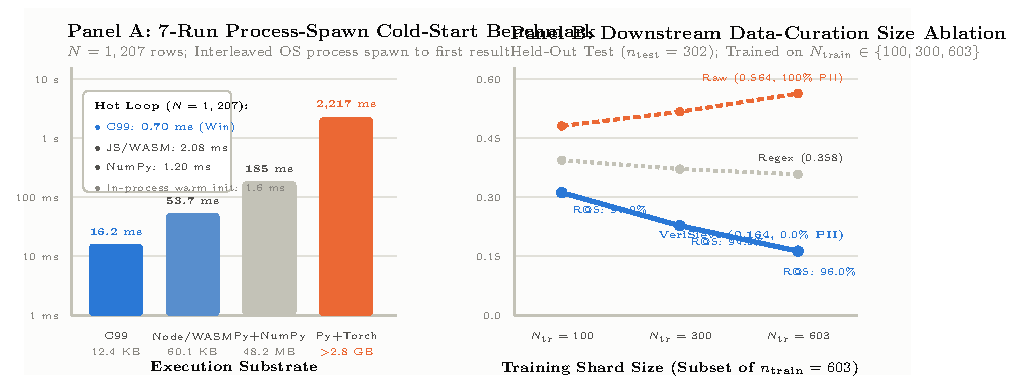
\includegraphics[width=0.96\textwidth]{figs/fig3-substrate-and-scaling.pdf}
\caption{Runtime substrate overhead and held-out learning curves. \textbf{Panel A:} Median OS process startup across $7$ interleaved runs (values in Table~\ref{tab:substrates}). \textbf{Panel B:} Held-out loss ($n_{\text{test}}=299$) as $N_{\text{train}}$ increases from $100$ to $607$ (values in Table~\ref{tab:ablation}); Needle R@5 stays at $60.0\%$.}
\label{fig:substrates}
\end{figure*}

\subsection{Process Startup vs.\ Warm Kernel Compute}
Interactive CLI tools, browser extensions, and MCP servers spawn short-lived processes, making cold startup latency and memory footprint first-order design constraints. Table~\ref{tab:substrates} reports the median of seven interleaved OS process spawns across four execution substrates (medians because first-boot page-cache outliers, $549.9$\,ms on C99 and $41.9$\,s on PyTorch, skew means).

\begin{table}[t]
\caption{Median of $7$ interleaved OS process spawns. Process startup and peak RSS are directly comparable across all rows; warm compute compares the shared $1{,}207{\times}520$ logistic kernel only between C99 and NumPy.}
\label{tab:substrates}
\vskip 0.08in
\begin{center}
\resizebox{\columnwidth}{!}{%
\begin{tabular}{lrrrrl}
\toprule
\textbf{Substrate} & \textbf{OS Spawn} & \textbf{Warm Work} & \textbf{Init/Import} & \textbf{Peak RSS} & \textbf{Warm Kernel} \\
\midrule
C99 header & $\mathbf{14.12}$\,ms & $0.745$\,ms & -- & $\mathbf{6.08}$\,MB & $1{,}207{\times}520$ logistic \\
Node.js + WASM & $106.22$\,ms & $7.125$\,ms & $1.045$\,ms & $55.97$\,MB & 64-d VeRA predict \\
Python + NumPy & $388.79$\,ms & $\mathbf{0.207}$\,ms & $187.01$\,ms & $31.49$\,MB & $1{,}207{\times}520$ logistic \\
Python + Torch + DuckDB & $12{,}917$\,ms & $31.47$\,ms & $11{,}662$\,ms & $432.3$\,MB & Qwen2 step, $100$ rows \\
\bottomrule
\end{tabular}%
}
\end{center}
\vskip -0.14in
\end{table}

Node.js+WASM starts $121.6\times$ faster than the PyTorch+DuckDB stack with $7.7\times$ lower peak RSS, and the standalone C99 binary is fastest of all; warm compute on the identical $1{,}207{\times}520$ float32 logistic dot product favors vectorized NumPy over scalar C99 (Table~\ref{tab:substrates}). The Node.js ($7.125$\,ms for 64-dimensional \texttt{mle\_dl\_vera\_predict} across two layers with JS readback) and PyTorch ($31.47$\,ms for a $100$-row Qwen2 forward/backward step) warm timings execute heavier neural workloads and are therefore not ranked against the linear dot product.

\subsection{Training Budget Scaling and WASM VeRA Convergence}
Varying the gate training shard size $N_{\text{train}} \in \{100, 300, 607\}$ on the disjoint $299$-document test split shows consistent improvement across both the linear gate and the WASM VeRA adapter (Table~\ref{tab:ablation}): binary cross-entropy (BCE) drops $26.7\%$ for the gate and, for VeRA, falls from above the $\ln 2 \approx 0.693$ constant-predictor baseline at $N_{\text{train}}=100$ down to $0.6141$ at $N_{\text{train}}=607$, with high-confidence contact leakage well inside the $\alpha=0.05$ budget. Across $125$ held-out PubMedQA retrieval queries, 64-dimensional Needle R@5 stays at $60.0\%$ (R@1 $31.2\%$) after Versieve redaction compared with $60.0\%$ raw (R@1 $32.0\%$) and $60.8\%$ naive regex, confirming that structured redaction preserves top-5 retrieval recall.

\begin{table}[t]
\caption{Held-out scaling ablation ($n_{\text{test}}=299$). Gate BCE measures the 520-dim logistic scorer; VeRA BCE measures \texttt{mle\_dl\_vera\_loss\_grad} in \texttt{versieve\_dl.wasm}.}
\label{tab:ablation}
\vskip 0.08in
\begin{center}
\resizebox{\columnwidth}{!}{%
\begin{tabular}{lrrrrr}
\toprule
\textbf{Pipeline ($N_{\text{train}}$)} & \textbf{Gate BCE} & \textbf{Gate Acc} & \textbf{VeRA BCE} & \textbf{PII Exposure} & \textbf{Needle R@5} \\
\midrule
Raw unfiltered & -- & $31.4\%$ & -- & $100\%$ & $60.0\%$ \\
Naive regex scrubber & $0.7833$ & $64.2\%$ & -- & Non-exempt & $60.8\%$ \\
\midrule
Versieve ($N_{\text{tr}}=100$) & $0.2577$ & $92\%$ & $0.9432$ & $0\%$ & -- \\
Versieve ($N_{\text{tr}}=300$) & $0.2244$ & $93\%$ & $0.6698$ & $0\%$ & -- \\
\textbf{Versieve ($N_{\text{tr}}=607$)} & $\mathbf{0.189}$ & $\mathbf{94\%}$ & $\mathbf{0.6141}$ & $\mathbf{1.05\%}$ & $\mathbf{60.0\%}$ \\
\bottomrule
\end{tabular}%
}
\end{center}
\vskip -0.14in
\end{table}

\subsection{Downstream Value of the Curated Outputs}
\label{sec:trackc}

Whether local open-weight models do better with fine-tuning on Versieve-curated text or with zero-training retrieval over it, and how PII redaction changes QA accuracy, adversarial leakage, and canary memorization, are measured in the companion local-training study \citep{ardiyansyah2026localtraining}, which reports the full Ollama CAG versus Graph-PPR comparison, the cross-family LoRA evaluation, and the canary-exposure measurements on the same hardware. This paper retains the substrate and training-budget scaling results above.

\section{Limitations and Operating Boundaries}
\label{sec:limitations}

Our experiments highlight five concrete boundaries that govern production deployment:
\begin{itemize}
    \item \textbf{Finite-sample calibration floor:} Certifying conditional LTT risk at $\alpha=0.01$ and $\delta=0.05$ mathematically requires at least $n_{\text{cal,unsafe}} \ge 299$. Smaller calibration sets trigger fail-closed abstention ($\tau_{\text{keep}}=1.0$), which preserves safety guarantees at the cost of automated throughput.
    \item \textbf{Certificate scope:} The unsafe and safe labels used for risk control are scanner-derived except where a dataset supplies ground-truth PII spans, so a certificate means agreement with the scanner family, not independent PII truth; the $31.0\%$ all-tag recall measures the scanner against \texttt{ai4privacy}'s human labels and bounds what the gate can catch.
    \item \textbf{Exchangeability assumption:} Learn-Then-Test guarantees assume that calibration and deployment shards are exchangeable; domain shifts require recalibration on fresh labeled samples.
    \item \textbf{Geometric survival vs.\ neural OCR accuracy:} The $97.38\%$ FUNSD result measures geometric box legibility under 2D tiling, not end-to-end character error rate from a neural OCR backbone.
    \item \textbf{Deterministic regex recall ceiling:} Format-validated regex misses roughly half of bare person names ($49.6\%$) and over-masks certain Title-Case legal phrases, a cost quantified in the companion training study \citep{ardiyansyah2026localtraining}. External NER taggers on the same $500$ records raise 26-tag recall to $64.48\%$ (Presidio) and $62.41\%$ (GLiNER-Edge), confirming most of the gap is regex-specific while over one third of structured spans still require conformal gatekeeping.
\end{itemize}

\section{Conclusion}
\label{sec:conclusion}

Versieve demonstrates that deterministic document parsing, salted-pseudonym redaction, and finite-sample conformal gatekeeping can run entirely inside a local sandbox with millisecond startup latency. Across $1{,}207$ public documents on an 8\,GB GPU, two system lessons stand out: (1)~deterministic regex must be paired with a fail-closed conformal gate, because format-validated rules recall only $31.0\%$ of structured PII spans overall and the certificates bound what the redaction layer can catch rather than independent PII truth; and (2)~where calibration is insufficient, fail-closed abstention is the correct output, trading automated throughput for a guarantee that only supported thresholds are certified. The downstream effects of the curated outputs are measured in the companion local-training study \citep{ardiyansyah2026localtraining}.

\bibliographystyle{mlsys2025}
\bibliography{versieve-extraction-redaction-benchmark}

\newpage
\appendix
\section{MCP Tool Interface and Zero-Egress WASM Verification}
\label{sec:mcp}

The local Model Context Protocol server (\texttt{src/mcp-server.js}) exposes $18$ JSON-RPC tools over stdio with zero user-byte egress:
\begin{itemize}
    \item \textbf{Curation and conformal gatekeeping ($8$ tools):} \texttt{ingest\_and\_tokenize}, \texttt{train\_local\_gatekeeper}, \texttt{gatekeeper\_decide}, \texttt{verify\_provenance\_chain}, \texttt{train\_multiaxis\_gatekeeper}, \texttt{gatekeeper\_decide\_multiaxis}, \texttt{ingest\_url\_or\_links}, and \texttt{plan\_local\_open\_weight\_training}.
    \item \textbf{Redacted knowledge graph and TOC ($6$ tools, \texttt{versieve\_graph.wasm}):} \texttt{index\_document\_graph}, \texttt{blast\_radius}, \texttt{ppr\_retrieve}, \texttt{trace\_path}, \texttt{get\_document\_tree}, and \texttt{read\_section\_nodes}.
    \item \textbf{Enterprise containers, secrets, audio, and forensics ($4$ tools, \texttt{versieve\_media.wasm}):} \texttt{ingest\_enterprise\_bundle}, \texttt{scan\_enterprise\_secrets}, \texttt{redact\_audio\_call}, and \texttt{audit\_forensic\_leaks}, evaluated in the companion multimodal study \citep{ardiyansyah2026multimodal}.
\end{itemize}

All five WebAssembly modules (\texttt{versieve\_dl.wasm} with $26$ \texttt{mle\_dl\_*} exports; $388{,}797$\,B combined; per-module sizes in Section~\ref{sec:intro}) pass automated SHA-256 provenance and zero-import verification (\texttt{npm run audit-wasm}: \texttt{allVerified = true}). The portable Node.js CI suite runs $226$ tests across $39$ test files ($215$ core tests plus $6$ MCP tests), alongside $4/4$ Python trainer unit tests in \texttt{test/versieve-train.test.py}.

\end{document}
